\documentclass[12pt,t]{beamer}

\usepackage[utf8]{inputenc} 
\usepackage[T1]{fontenc}
\usepackage{lmodern}
\usepackage{graphicx}
\usepackage[english]{babel}
\usepackage[absolute,overlay]{textpos}
\usepackage{epstopdf}
\usepackage{tikz}
\usetikzlibrary{shapes}
 
%\usetheme{Madrid}
%\usetheme{CambridgeUS}
\usetheme[noflama]{hsrm} 

%\usefonttheme{professionalfonts}
%\usefonttheme{serif}

%\setbeamercolor{footline}{fg=blue}
%\setbeamerfont{footline}{series=\bfseries}
\setbeameroption{show notes}

\title[Study of Sintered BMG]{Atomistic Study of the Mechanical Properites of a Sintered Bulk Metallic Glass (Nanoglass)}
\author[Ardiani (francoamg@gmail.com)]{Franco Ardiani$^a$ (francoamg@gmail.com), Andr\'es A. Manelli$^a$, Carlos J. Ruestes$^{b,c}$, Claudio A. Careglio$^{a}$ and Eduardo M. Bringa$^{b,c}$}
\institute[UNCUYO]{$^a$Facultad de Ingenier\'ia, Universidad Nacional de Cuyo\\$^b$FCEN, Universidad Nacional de Cuyo\\$^c$CONICET}
\date{\today}


\begin{document}

%%%
% Slide de titulo y contenidos
%%%

\begingroup
\makeatletter
\makeatother
\begin{frame}[plain]
    \maketitle
    \begin{textblock*}{12cm}(0.5cm,8.5cm) % {block width} (coords)
        \tiny{Acknowledgements:\\ We thank support from SeCTyP-UNCuyo grant B008. EMB and CJR also thank support from PICT-PRH 0092.}
    \end{textblock*}
    \begin{textblock*}{1.5cm}(10.5cm,6.3cm) % {block width} (coords)
        
\includegraphics[width=1.5cm]{Presentacion_PANACM_Franco/fing.png}
    \end{textblock*}
    \begin{textblock*}{2cm}(0.5cm,5.8cm) % {block width} (coords)
        
\includegraphics[width=2cm]{Presentacion_PANACM_Franco/uncuyo.jpg}
    \end{textblock*}
    \begin{textblock*}{2cm}(0.7cm,6.8cm) % {block width} (coords)
        
\includegraphics[width=2cm]{Presentacion_PANACM_Franco/logofcen3.png}
    \end{textblock*}
\end{frame}
\endgroup

\begin{frame}
   \frametitle{Contents}
   \tableofcontents[currentsection,sectionstyle=show,subsectionstyle=show/shaded/hide]
\end{frame}

%%%
% Introduccion
%%%

\section{Introduction}

\begin{frame}
    \frametitle{Introduction}
    \vspace{0.2cm}
    \begin{itemize}
        \item Metallic Glass: amorphous metal (without crystalline order).
        \item Has advantages over crystalline metals, like elasticity combined with high resistance, strength and moldability.
        \item Plasticity in these materials occurs by nucleation of shear transformation zones which grow into shear bands.
        \item Shear bands may lead to brittle failure (heterogeneous deformation): importance of \textbf{preventing their propagation}.
        \item A more homogeneous deformation may be achieved by adding \textbf{porosity}.
    \end{itemize} 
\end{frame}

\note{
    \begin{textblock*}{11.5cm}(0.5cm,2.5cm) 
        \begin{itemize}
            \item Example applications for MGs: amorphous structural steels, biomedical materials, aerospace materials, etc.
            \item Production of MGs: techniques which include high quenching rates, low volumes and composition control.
            \item STZs and SBs: STZs are small zones of intense shearing strain, consisting of a few atoms. A SB contains more atoms and has a different aspect ratio.
            \item Porosity to evitate the propagation of SBs: related to the way of preventing dislocation motion in metals.
            \item MD (Molecular Dynamics): solves problems with many atoms, interacting through an interatomic potential or force field.
        \end{itemize} 
    \end{textblock*}
 }

%%%
% Detalles de la simulacion
%%%

\section{Simulation details}

\begin{frame}
    \frametitle{Simulation details}
    \vspace{0.2cm}
    \begin{itemize}
        \item Software: Lammps (lammps.sandia.gov) for simulation, Ovito (www.ovito.org) and Gnuplot for analysis.
        \item Sample: based on Cu$_{46}$ Zr$_{54}$ described by Arman et al. (2010).
        \begin{itemize}
            \item Cooling rate 10$^{12}$ K/s.
        \end{itemize}
        \item EAM (Embedded Atom Method; Daw, 1984) alloy potential adopted (Cheng, 2008).
    \end{itemize}
    \begin{textblock*}{12cm}(0.5cm,6.5cm) % {block width} (coords)
        \small{Arman B., Luo S.-N., Germann T.C. and Cağin T., \textit{Phys. Rev. B.}, \textbf{81}, 144201 (2010).\\
        Daw M. and Baskes M.I., \textit{Phys. Rev. B.}, \textbf{29}:6443-6453 (1984).\\
        Cheng Y.Q., Sheng H.W. and Ma E., \textit{Phys. Rev. B.}, \textbf{78}, 014207 (2008) https://sites.google.com/site/eampotentials/}
    \end{textblock*}
\end{frame}

\note{
    \begin{textblock*}{10.6cm}(1.8cm,5cm) 
        \begin{itemize}
            \item EAM: the total energy $E_i$ of an atom $i$ is given by this equation, where F is the embedding energy which is a function of the atomic electron density $\rho$, $\phi$ is a pair potential interaction, and $\alpha$ and $\beta$ are the element types of atoms I and J. The multi-body nature of the EAM potential is a result of the embedding energy term. Both summations in the formula are over all neighbors J of atom I within the cutoff distance.
        \end{itemize}
    \end{textblock*}
    \begin{exampleblock}{EAM}
        \[
            E_i=F_{\alpha} \left ( \sum \limits_{i\neq j} \rho _{\beta} (r_{ij}) \right ) + \frac{1}{2} \sum \limits_{i\neq j} \phi _{\alpha \beta} (r_{ij})
        \]
    \end{exampleblock}
}

%\note{
%    \begin{textblock*}{10.6cm}(1.8cm,5cm) 
%        \begin{itemize}
%            \item EAM: the potential energy of an atom, $i$, is given by this equation, where $r_{ij}$ is the distance between atoms $i$ and $j$, $\phi_{\alpha\beta}$ is a pair-wise potential function, $\rho_\beta$ is the contribution to the electron charge density from atom $j$ of type $\beta$ at the location of atom $i$, and $F$ is an embedding function that represents the energy required to place atom $i$ of type $\alpha$ into the electron cloud.
%        \end{itemize}
%    \end{textblock*}
%    \begin{exampleblock}{EAM}
%        \[
%            E_i=F_{\alpha} \left ( \sum \limits_{i\neq j} \rho _{\beta} (r_{ij}) \right ) + \frac{1}{2} \sum \limits_{i\neq j} \phi _{\alpha \beta} (r_{ij})
%        \]
%    \end{exampleblock}
%}

%%%
% Preparacion de la muestra
%%%

\section{Porous sample preparation}

\begin{frame}
    \frametitle{Porous sample preparation}
    \framesubtitle{Procedure}
    \vspace{0cm}
    \begin{enumerate}
        \item Random placement of 2.5 nm radius spheres.
        \item Relaxation @ 650K (constant volume, few ps). 
        \item Up to 10 ps of compressive pressure (400 bar).
        \item Repeat two previous steps.
        \item Further relaxation: cooling to zero T, barostat to zero pressure, heating to simulation temperature and, barostat to zero pressure (5 ps, constant T)
        \begin{textblock*}{3cm}(2.5cm,6.5cm) % {block width} (coords)
            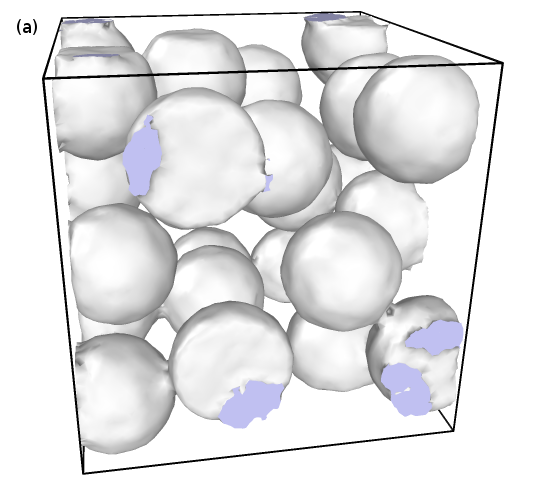
\includegraphics[width=3cm]{Presentacion_PANACM_Franco/spheres2.png}
        \end{textblock*}
        \begin{textblock*}{3cm}(7cm,6.5cm) % {block width} (coords)
            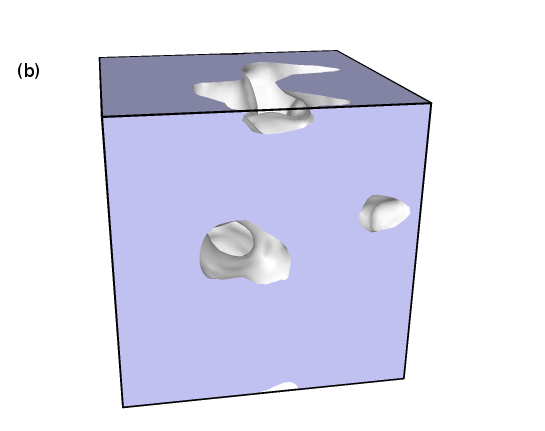
\includegraphics[width=3cm]{Presentacion_PANACM_Franco/spheres3.png}
        \end{textblock*}
    \end{enumerate}
\end{frame}

%%%
% Resultados
%%%

\section{Results}

\begin{frame}
    \frametitle{Results}
    \framesubtitle{Samples and loading}
    \vspace{1cm}
    \begin{itemize}
        \item Took samples of different initial porosities (3.3\%, 5.8\% and 13.1\%).
        \item Loading at a strain rate of 10$^9/s$, appropiate for shock compression experiments.
        \item Purely uniaxial strain.
        \item Periodic boundary conditions.
    \end{itemize}
\end{frame}

\begin{frame}
    \frametitle{Results}
    \framesubtitle{Compression}
    \begin{textblock*}{7.5cm}(0.3cm,2cm) % {block width} (coords)
        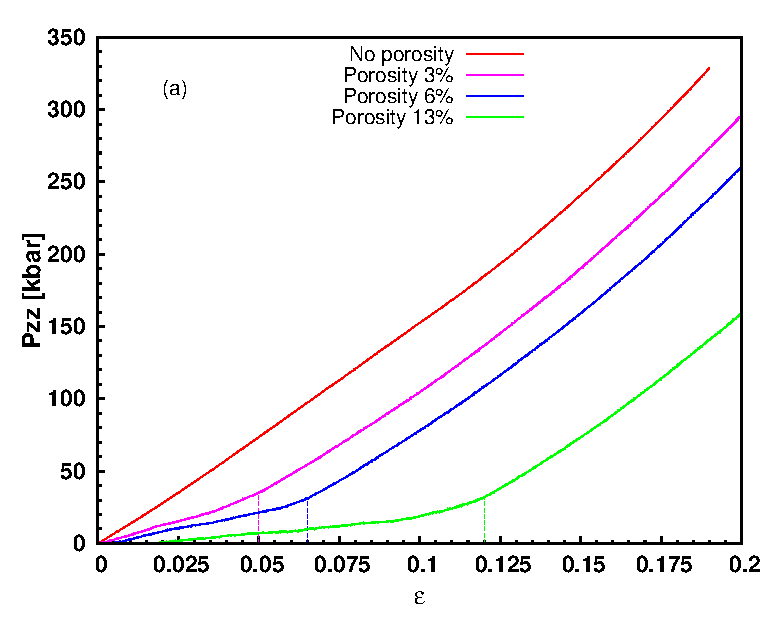
\includegraphics[width=7.5cm]{Presentacion_PANACM_Franco/Pzz_strain_comp_dash.eps}
    \end{textblock*}
    \begin{textblock*}{4.2cm}(0.6cm,6.75cm) % {block width} (coords)
        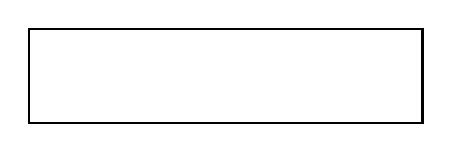
\begin{tikzpicture}
            \draw[thick] (0,0) rectangle (5cm,1.2cm);
        \end{tikzpicture}
    \end{textblock*}
    \begin{textblock*}{5cm}(7.86cm,2.5cm) % {block width} (coords)
        After pore closure, curves are similar to the one for no porosity. There is significant hardening after pore closure.
    \end{textblock*}
    \begin{textblock*}{5cm}(7.86cm,5.8cm) % {block width} (coords)
        Before pore closure, strain increases while maintaining low stress levels.\\
        Porosity produces shear concentration, and pores start to collapse.
    \end{textblock*}
\end{frame}

\begin{frame}
    \frametitle{Results}
    \framesubtitle{Compression}
    \begin{textblock*}{6.5cm}(0.4cm,2cm) % {block width} (coords)
        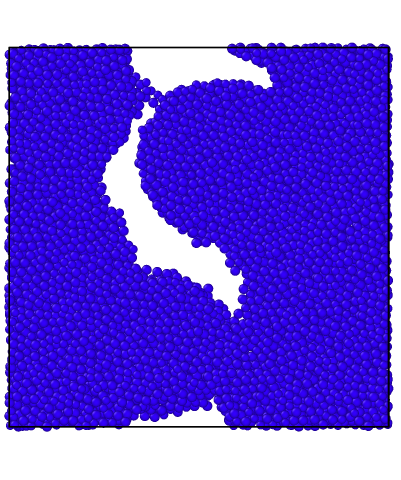
\includegraphics[width=4cm]{Presentacion_PANACM_Franco/13_0strain.png}
        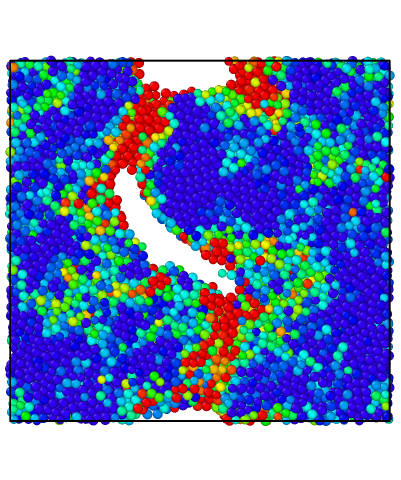
\includegraphics[width=4cm]{Presentacion_PANACM_Franco/13_5strain_comp.png}
        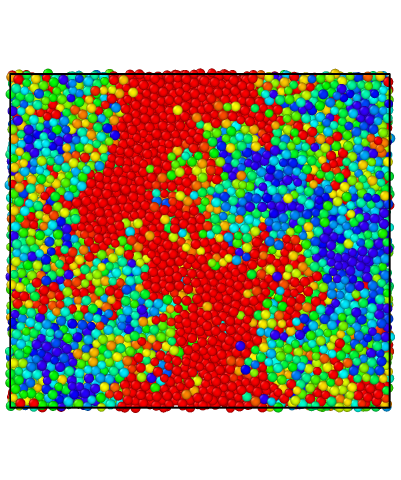
\includegraphics[width=4cm]{Presentacion_PANACM_Franco/13_12strain_comp.png}
    \end{textblock*}
    \begin{textblock*}{11cm}(1.2cm,6.4cm) % {block width} (coords)
        \centering
        \tiny{Shear strain coloring for a thin slice of the 13\% porosity sample. Strains are 0, 5 and 12\%\\Blue correspondes to shear strain lower than 10\%, and red to shear strain greater than 30\%}
    \end{textblock*}
    \begin{textblock*}{11cm}(1cm,7.1cm) % {block width} (coords)
        Pores act as stress concentrators.\\
        They also impede incipient shear band formation.\\
        Accumulation of strain along diagonal directions, as in incipient shear banding.
    \end{textblock*}
\end{frame}

\begin{frame}
    \frametitle{Results}
    \framesubtitle{Compression}
    \begin{textblock*}{7.5cm}(0.3cm,2cm) % {block width} (coords)
        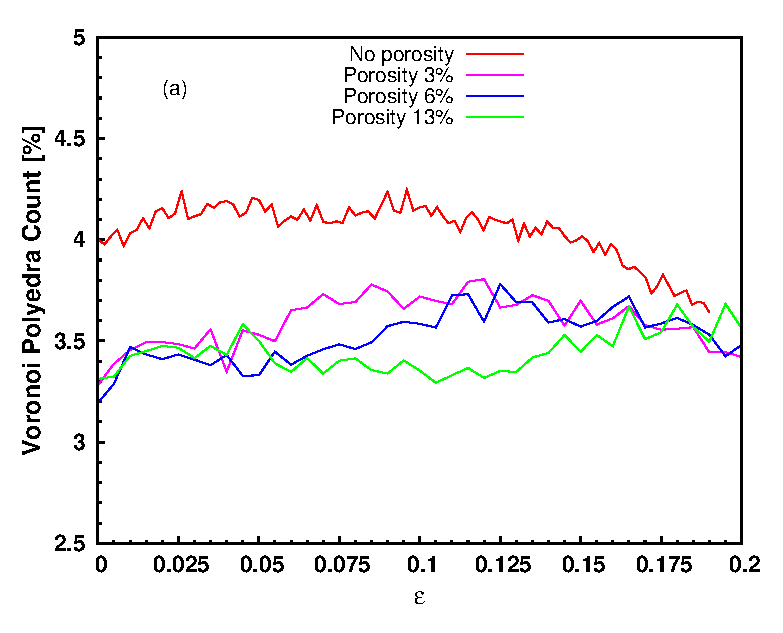
\includegraphics[width=7.5cm]{Presentacion_PANACM_Franco/tipe3_strain_comp.eps}
    \end{textblock*}
    \begin{textblock*}{5cm}(7.9cm,2.5cm) % {block width} (coords)
        The fall in the number of Type 3 atoms after a constant stage has been thought to be an indicator of the onset of plasticity (Arman, 2010).
    \end{textblock*}
    \begin{textblock*}{5cm}(8cm,5.8cm) % {block width} (coords)
        Counter-intuitive result.\\
        Here we do have plasticity but there is almost no change in Voronoi polyhedra.\\
        Other processes involved?
    \end{textblock*}
\end{frame}

\note{
    \begin{textblock*}{6.5cm}(2.5cm,2.5cm) % {block width} (coords)
        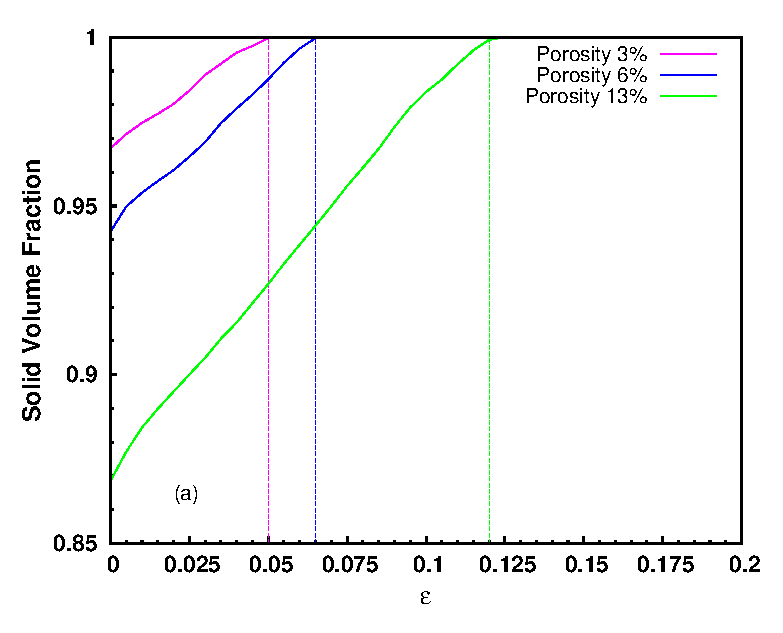
\includegraphics[width=6.5cm]{Presentacion_PANACM_Franco/SVF_strain_comp_dash.eps}
    \end{textblock*}
    \begin{textblock*}{3cm}(9.2cm,3cm) % {block width} (coords)
        Solid volume fraction versus strain.
    \end{textblock*}
    \begin{textblock*}{9cm}(2.8cm,7.9cm) % {block width} (coords)
        The dashed lines show when pores totally close. The values are: \\
        $3\% \rightarrow 0.05, 6\% \rightarrow 0.065, 13\% \rightarrow 0.12$
    \end{textblock*}
}

\note{
    \begin{textblock*}{6.5cm}(2.5cm,2.5cm) % {block width} (coords)
        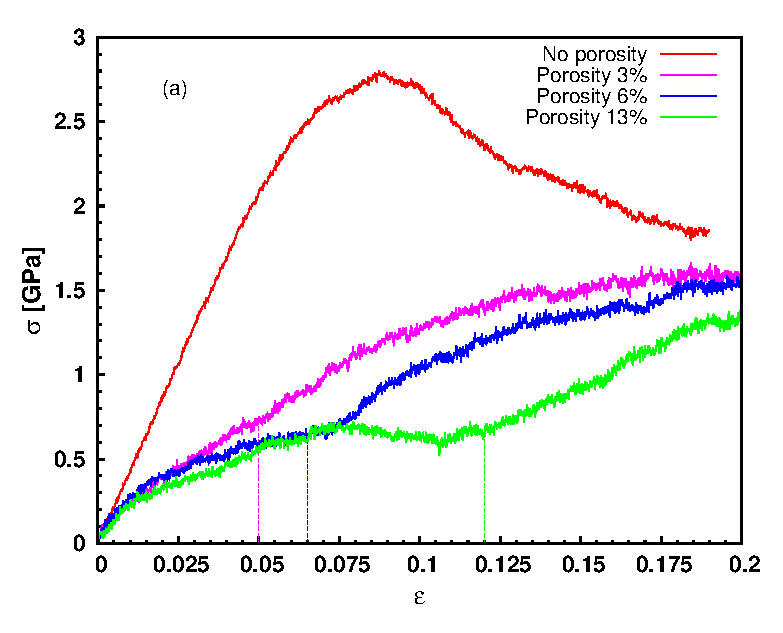
\includegraphics[width=6.5cm]{Presentacion_PANACM_Franco/stress_strain_comp_dash.eps}
    \end{textblock*}
    \begin{textblock*}{3cm}(9.2cm,3cm) % {block width} (coords)
        Von Mises stress versus strain.
    \end{textblock*}
    \begin{textblock*}{9cm}(2.8cm,8.2cm) % {block width} (coords)

    \end{textblock*}
}

\begin{frame}
    \frametitle{Results}
    \framesubtitle{Tension}
    \begin{textblock*}{7.5cm}(0.3cm,2cm) % {block width} (coords)
        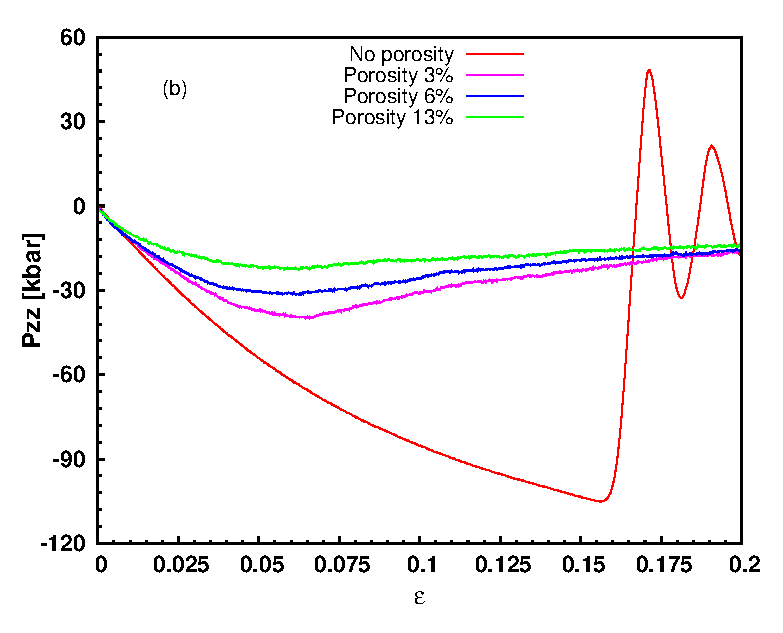
\includegraphics[width=7.5cm]{Presentacion_PANACM_Franco/Pzz_strain_tens.eps}
    \end{textblock*}
    \begin{textblock*}{4cm}(8cm,2.2cm) % {block width} (coords)
        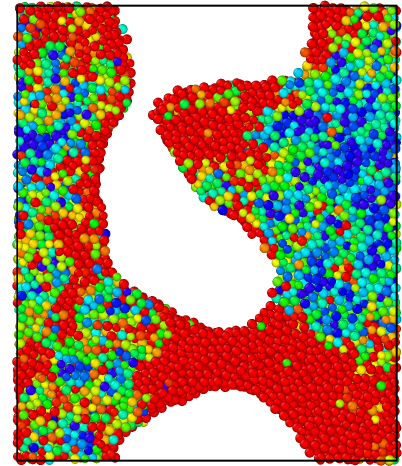
\includegraphics[width=4cm]{Presentacion_PANACM_Franco/13_20strain_tens.png}\\
        \centering
        \tiny{Shear strain coloring of the 13\% porosity sample’s slice at 20\% strain.}
    \end{textblock*}
    \begin{textblock*}{11.5cm}(0.5cm,7.8cm) % {block width} (coords)
        Plastic flow.\\
        The use of periodic boundary conditions precludes the closing of the voids (there is no necking).
    \end{textblock*}
\end{frame}

\begin{frame}
    \frametitle{Results}
    \framesubtitle{Tension}
    \begin{textblock*}{6.5cm}(0.4cm,2cm) % {block width} (coords)
        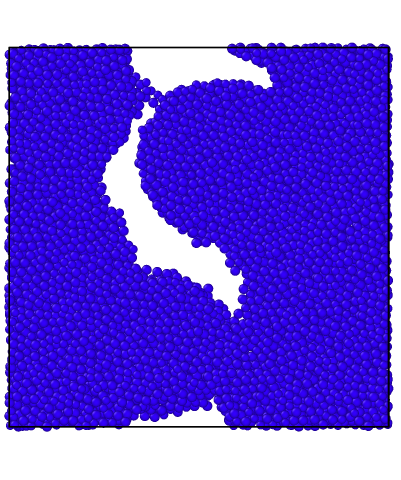
\includegraphics[width=4cm]{Presentacion_PANACM_Franco/13_0strain.png}
        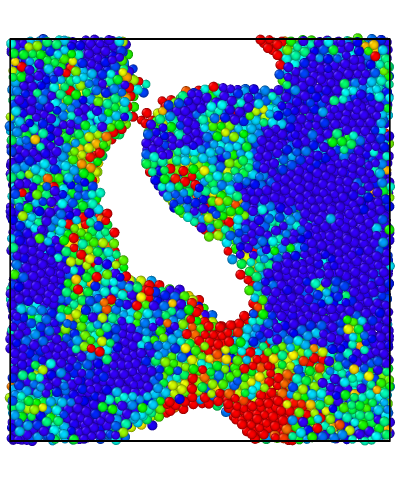
\includegraphics[width=4cm]{Presentacion_PANACM_Franco/13_6strain_tens.png}
        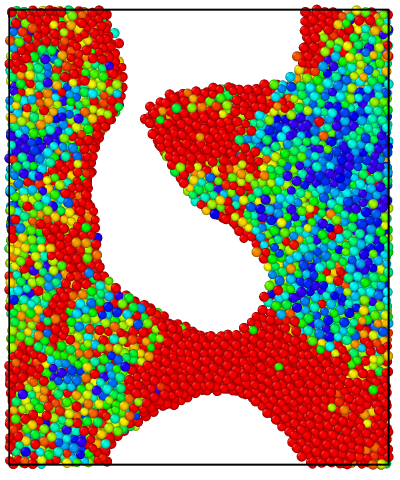
\includegraphics[width=4cm]{Presentacion_PANACM_Franco/13_20strain_tens_2.png}
    \end{textblock*}
    \begin{textblock*}{11cm}(1cm,7cm) % {block width} (coords)
        \centering
        \tiny{Shear strain coloring of a thin slice of the 13\% porosity sample. Strains are 0, 6 and 20\%\\Blue correspondes to shear strain lower than 10\%, and red to shear strain greater than 30\%}
    \end{textblock*}
    \begin{textblock*}{11.5cm}(1cm,8cm) % {block width} (coords)
        Shear strain is mostly concentrated around the pores.
%            \item Relative position between atoms remains almost the same.
    \end{textblock*}
\end{frame}

\begin{frame}
    \frametitle{Results}
    \framesubtitle{Tension}
    \begin{textblock*}{7.5cm}(0.3cm,2cm) % {block width} (coords)
        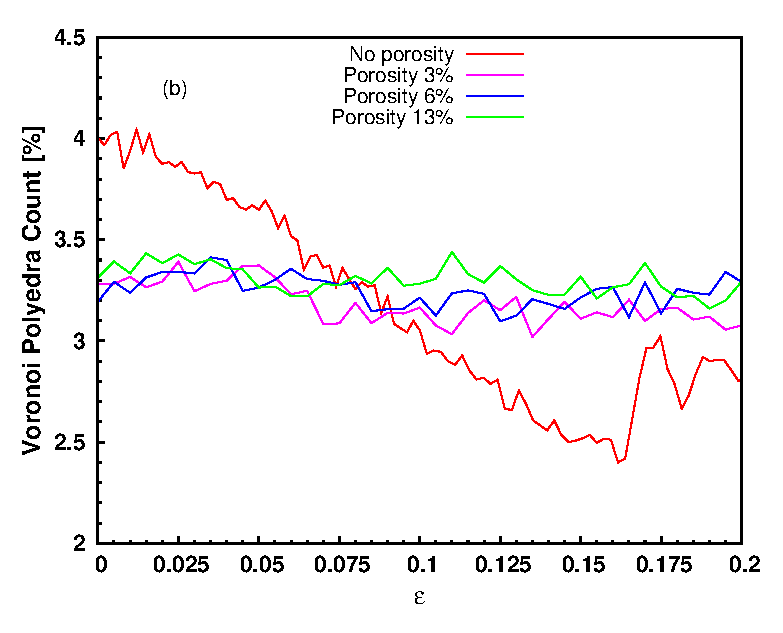
\includegraphics[width=7.5cm]{Presentacion_PANACM_Franco/tipe3_strain_tens.eps}
    \end{textblock*}
    \begin{textblock*}{4.2cm}(6.7cm,4cm) % {block width} (coords)
        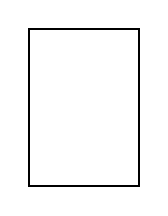
\begin{tikzpicture}
            \draw[thick] (0,0) rectangle (1.4cm,2cm);
        \end{tikzpicture}
    \end{textblock*}
    \begin{textblock*}{5cm}(8cm,3cm) % {block width} (coords)
        Constant after void nucleation.
    \end{textblock*}
    \begin{textblock*}{12cm}(0.4cm,7.9cm) % {block width} (coords)
        There is significant motion of atoms around pores, preventing the formation of STZs other than the ones around the pores.
    \end{textblock*}
\end{frame}

\note{
    \begin{textblock*}{6.5cm}(2.5cm,2.5cm) % {block width} (coords)
        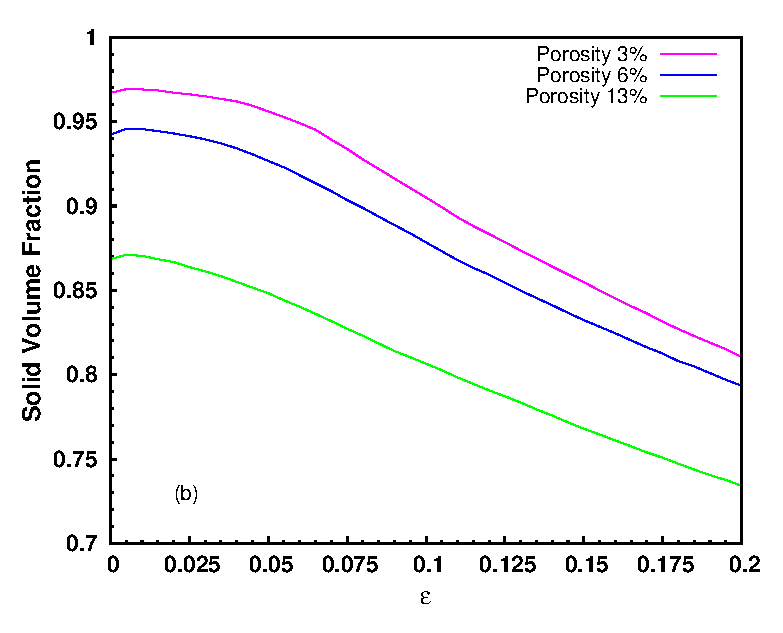
\includegraphics[width=6.5cm]{Presentacion_PANACM_Franco/SVF_strain_tens.eps}
    \end{textblock*}
    \begin{textblock*}{3cm}(9.2cm,3cm) % {block width} (coords)
        Solid volume fraction versus strain.
    \end{textblock*}
}

\note{
    \begin{textblock*}{6.5cm}(2.5cm,2.5cm) % {block width} (coords)
        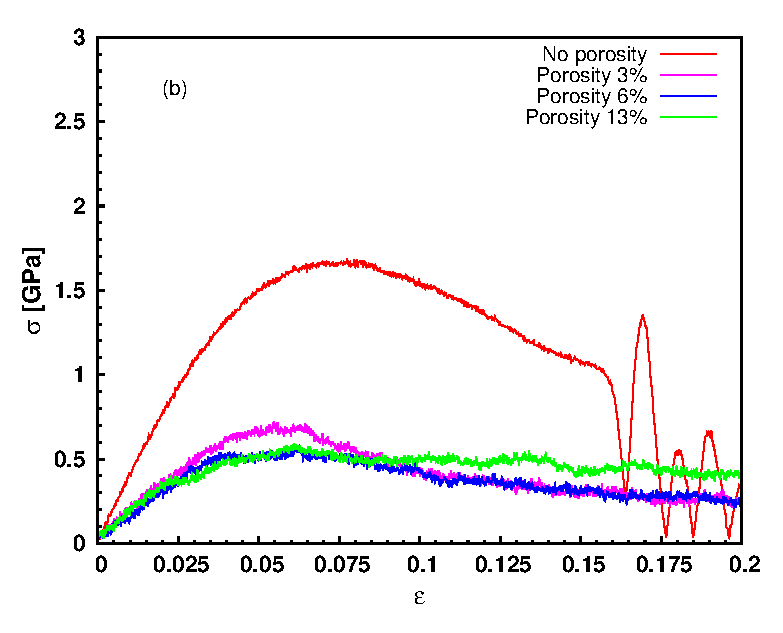
\includegraphics[width=6.5cm]{Presentacion_PANACM_Franco/stress_strain_tens.eps}
    \end{textblock*}
    \begin{textblock*}{3cm}(9.2cm,3cm) % {block width} (coords)
        Von Mises stress versus strain.
    \end{textblock*}
    \begin{textblock*}{9cm}(2.8cm,8.2cm) % {block width} (coords)

    \end{textblock*}
}

%%%
% Conclusiones
%%%

\section{Conclusions}

\begin{frame}
    \frametitle{Conclusions}
    \vspace{0.5cm}
    \begin{itemize}
        \item Sintering process leads to glass with taylored porosity values.
        \item Under compression: pores act as stress concentrators but also delay nucleation of SBs. After closure, there is hardening.
        \item Under tension: pores do not close and they concentrate plastic flow around them, also impeding formation of STZ and SBs.
        \item Results under strain were somewhat comparable to the ones by Yuan et al. (2014), where a single crystal sample with voids was studied.
    \end{itemize}
    \begin{textblock*}{12cm}(1cm,8.2cm) % {block width} (coords)
        \small{Yuan F. and Wu X., \textit{AIP ADVANCES}, \textbf{4}, 127109 (2014).}
    \end{textblock*}
\end{frame}

\note{
    \begin{textblock*}{5cm}(2cm,3.2cm) % {block width} (coords)
        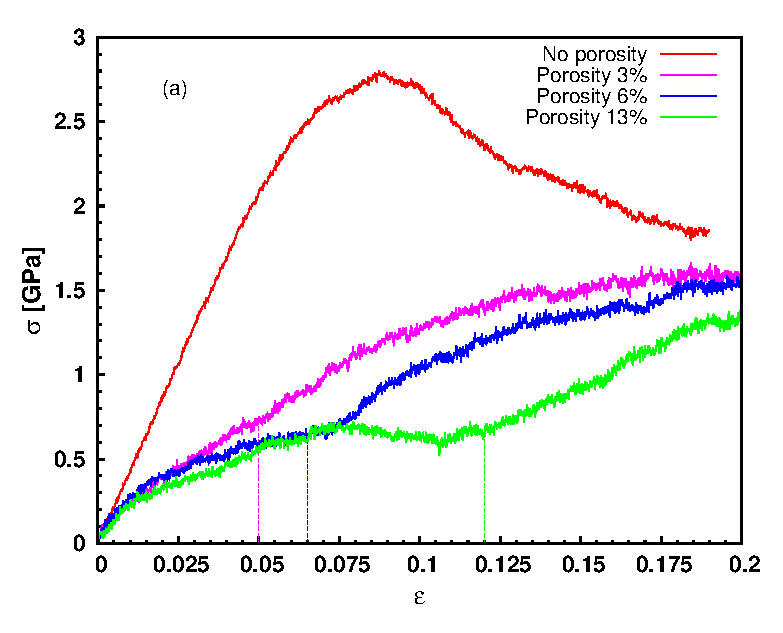
\includegraphics[width=5cm]{Presentacion_PANACM_Franco/stress_strain_comp_dash.eps}
    \end{textblock*}
    \begin{textblock*}{3cm}(7cm,3cm) % {block width} (coords)
        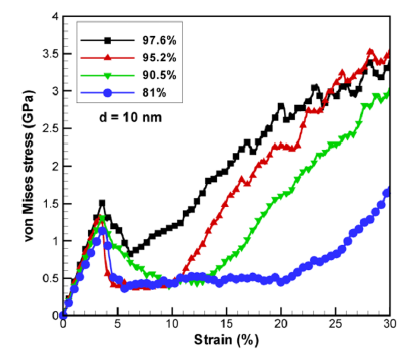
\includegraphics[width=5cm]{Presentacion_PANACM_Franco/Yuan_VM.png}
    \end{textblock*}
    \begin{textblock*}{12cm}(1cm,8.2cm) % {block width} (coords)
        \small{Yuan F. and Wu X., \textit{AIP ADVANCES}, \textbf{4}, 127109 (2014).}
    \end{textblock*}
}

\note{
    \begin{textblock*}{5cm}(2cm,3.2cm) % {block width} (coords)
        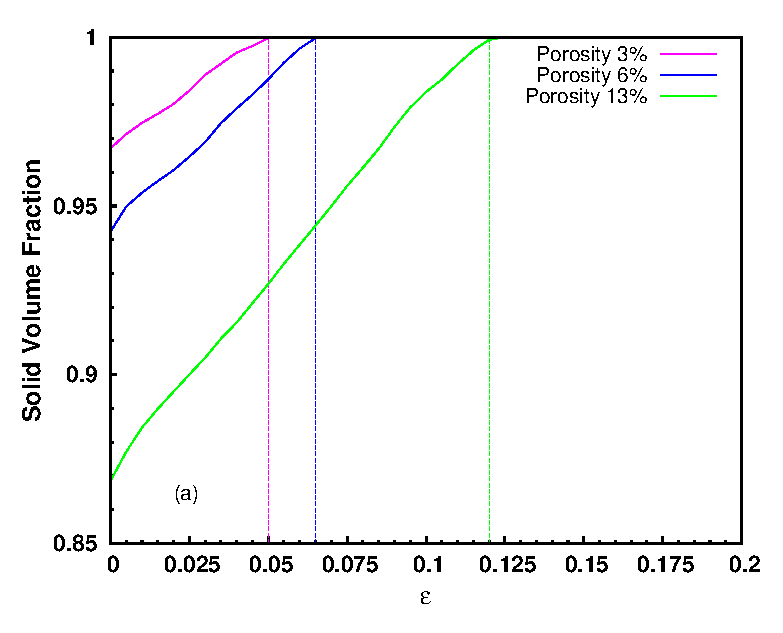
\includegraphics[width=5cm]{Presentacion_PANACM_Franco/SVF_strain_comp_dash.eps}
    \end{textblock*}
    \begin{textblock*}{3cm}(7cm,3cm) % {block width} (coords)
        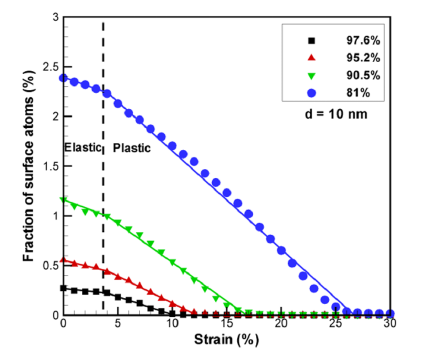
\includegraphics[width=5cm]{Presentacion_PANACM_Franco/Yuan_SVF.png}
    \end{textblock*}
    \begin{textblock*}{12cm}(1cm,8.2cm) % {block width} (coords)
        \small{Yuan F. and Wu X., \textit{AIP ADVANCES}, \textbf{4}, 127109 (2014).}
    \end{textblock*}
}

%%%
% Slide de titulo
%%%

\begingroup
\makeatletter
\makeatother
\begin{frame}[plain]
    \maketitle
    \begin{textblock*}{12cm}(0.5cm,8.5cm) % {block width} (coords)
        \tiny{Acknowledgements:\\ We thank support from SeCTyP-UNCuyo grant B008. EMB and CJR also thank support from PICT-PRH 0092.}
    \end{textblock*}
    \begin{textblock*}{1.5cm}(10.5cm,6.3cm) % {block width} (coords)
        
\includegraphics[width=1.5cm]{Presentacion_PANACM_Franco/fing.png}
    \end{textblock*}
    \begin{textblock*}{2cm}(0.5cm,5.8cm) % {block width} (coords)
        
\includegraphics[width=2cm]{Presentacion_PANACM_Franco/uncuyo.jpg}
    \end{textblock*}
    \begin{textblock*}{2cm}(0.7cm,6.8cm) % {block width} (coords)
        
\includegraphics[width=2cm]{Presentacion_PANACM_Franco/logofcen3.png}
    \end{textblock*}
\end{frame}
\endgroup

\end{document}
